%\begin{abstract}

 %   The  \ion{Mg}{2}~k \& h line intensity ratios can be used to probe the characteristics of the plasma in the solar atmosphere. In this study, using the observations recorded by the Interface Region Imaging Spectrometer (IRIS), we study the variation of the  \ion{Mg}{2}~k \& h intensity ratio for three flares belonging to X-class, M-class, and C-class, throughout their evolution. We also study the k-to-h intensity ratio as a function of magnetic flux density obtained from the line-of-sight magnetograms recorded by the Helioseismic and Magnetic Imager (HMI) on board the Solar Dynamics Observatory (SDO). Our results reveal that while the intensity ratios are independent of magnetic flux density, they show significant changes during the evolution of the C-class and M-class flares. The intensity ratios start to increase at the start of the flare and peak during the impulsive phase before the flare peak and decrease rapidly thereafter. The values of the ratios fall even below the pre-flare level during the peak and decline phases of the flare. These results are important in the light of heating and cooling of localized plasma and provide further constraint on the understanding of flare physics.
    
%\end{abstract}
\justifying

%%----------------------------------------------------
\section{Introduction} \label{sec:intro}
%%----------------------------------------------------

Solar flares are the most energetic events on the Sun, where an enormous amount of magnetic free energy is released due to the reconfiguration of the coronal magnetic field. The released energy can cause particle acceleration, heating and flows in the solar atmosphere and a transient enhancement in solar radiative output. Notably, a significant portion of the radiated energy during flares originates from the dense chromosphere \citep{fletcher10,milligan14}. Therefore, examining chromospheric lines during flares offers valuable diagnostic tools for understanding the physics of solar flares and their impact on the local plasma environment.

The chromosphere emits radiation across various ultraviolet (UV) and optical lines. While many optical lines, such as H$\alpha$ and \ion{Ca}{2}, are routinely observed from ground-based telescopes, observations of the  \ion{Mg}{2} resonance lines have been relatively infrequent in the past. However, since the launch of the Interface Region Imaging Spectrograph (IRIS) \citep{iris}, regular monitoring of these lines with excellent spatial and spectral resolution has become possible.

The  \ion{Mg}{2} k and h lines represent transitions to the ground state from finely split upper levels ($3p~^{2}P_{\nicefrac{3}{2}}${--}$3s~^{2}S_{\nicefrac{1}{2}}$ and $3p ^{2}P_{\nicefrac{1}{2}}${--}$3s^{2}S_{\nicefrac{1}{2}}$), resulting in optically thick lines at wavelengths 2796.34~{\AA} ( \ion{Mg}{2} k) and 2803.52{\AA} ( \ion{Mg}{2} h). It has been suggested that the intensity ratios of these lines can offer insights into the optical depth of the local environment \citep{kerr15}.

The integrated intensity of a line transitioning from an upper level $j$ to a lower level $i$ depends on the collision strength $\Omega_{ij}$ for that transition, given by~\citep{henri62,mariska92},

%%---------------------------------------------------------------
\begin{equation*}
\Omega_{ij}=\frac{8\pi}{\sqrt{3}}~\frac{I_{H}}{\Delta \epsilon_{ij}}g\omega_{i}~f_{ij}
\end{equation*}
%%---------------------------------------------------------------

\noindent Here, $I_{H}$ denotes the ionization energy of hydrogen, $\Delta \epsilon_{ij}$ represents the threshold energy for the transition, $g$ is the Gaunt factor, $\omega_{i}$ is the statistical weight of the level, and $f_{ij}$ stands for the oscillator strength. In optically thin conditions, the intensity ratio of the k to h line equals the ratio of collision strengths, as the escape probability of photons is unity. As the  \ion{Mg}{2} k and h lines share the same ionization state and originate from a transition to a shared lower level, and given that the statistical weight ($\omega_{i}$) is the same in both cases, the line intensity ratio is simply the ratio of oscillator strengths ($f_{ij}$). Consequently, this ratio is expected to be 2:1 in optically thin conditions and lower when the medium is optically thick \citep{kerr15,levens19}.

Moreover, the  \ion{Mg}{2} k and h lines can serve to estimate velocity in the middle and upper chromosphere, chromospheric velocity gradients, and temperature in the middle chromosphere \citep{leenarts13a,leenarts13b,pereira13}. Emission from the  \ion{Mg}{2} triplets can help identify heating in the lower chromosphere \citep{pereira15}. Various studies have demonstrated spatial variations in  \ion{Mg}{2} line profiles \citep{dalda23,panos18}. For instance, \cite{polito23} associated the leading edge of flare ribbons with enhanced broadening and strong central reversal, interpreting this difference in profile as indicative of distinct heating mechanisms at different locations within flare ribbons. Similarly, \cite{panos21,panos21_2} revealed differences in line profiles and energy input.

Using observations recorded by the OSO-8 LPSP instrument, \citep{lemaire84} investigated the evolution of intensity ratios of  \ion{Mg}{2} h \& k, \ion{Ca}{2} h \& k, and Ly$\alpha$ \&~$\beta$ lines. They observed that the intensity ratio of the \ion{Ca}{2}~k/h lines increased from 1 to 1.2 during the ascending phase of a flare and returned to 1 during later phases. This correlated temporal behavior across various elements was interpreted as an indication of downward energy propagation, suggesting a potential decrease in opacity due to localized heating at the formation height of the \ion{Ca}{2} line during the flare's rise phase.

Here, we investigate the evolution of intensity ratios of the  \ion{Mg}{2} h \& k lines during three flares: C-class, M-class, and X-class. Specifically, we focus on the dependence of line ratios on the underlying magnetic field strength, a relationship that, to our knowledge, has not been explored previously. The remainder of this chapter is organized as follows. Section \ref{sec:obs} presents the observations utilized in this study, followed by our data reduction and analysis methods, and the results in Section \ref{sec:dar}.

%%----------------------------------------------------
\section{Observations} \label{sec:obs}
%%----------------------------------------------------
%%-------------------------------------------------------
\begin{table*}[ht!]
\centering
\resizebox{0.9\textwidth}{!}{%
\begin{tabular}{|c|c|c|c|c|c|}
\hline
Event & Flare & Flare & Raster & Raster Step & Raster \\
Date & Peak (UT) & Location (arcsec) & Details & (arcsec) & Cadence (s)\\
\hline
Nov 4, 2015  & 13:52 & [37",61"] & Coarse & 2" & 50\\
(M-class) & & & 16-step  & & \\
 & & & & & \\
Oct 22, 2014 & 14:28 & [-292",-302"] & Coarse & 2" & 131\\
(X-class) & & & 8-step  & & \\
 & & & & & \\
Feb 3, 2015 & 22:55 & [198",213"] & Dense & 0.35" & 33\\
(C-class) & & & 16-step  & & \\
\hline
\end{tabular}}
%\end{center}
\caption{List of flares studied in this chapter.}
\label{tab:my_label}
\end{table*}
%%-------------------------------------------------------

For this study, we selected three flares of M, X, and C classes, as listed in Table~\ref{tab:my_label} by IRIS. IRIS is a NASA small explorer-class solar observation satellite that obtains UV spectra with high spatial (0.33{--}0.4\arcsec per pixel), temporal (1s), and spectral resolution ($\sim$26 and $\sim$53~m{\AA}). The primary lines regularly observed by IRIS include \ion{C}{2},  \ion{Mg}{2}, and \ion{Si}{4}. In the imaging channel, it typically observes in  \ion{Mg}{2} and \ion{Si}{4}. In our study, we utilized observations recorded in the  \ion{Mg}{2} h\& k lines.

As mentioned earlier, this study aims to analyze the evolution of intensity ratios concerning magnetic flux density during the flares of various classes. To achieve this, we incorporated line-of-sight (LOS) magnetic field measurements from the Helioseismic and Magnetic Imager \citep[HMI;][]{hmi} on the Solar Dynamics Observatory \citep[SDO;][]{sdo}. We utilized observations taken at 1600~{\AA} by the Atmospheric Imaging Assembly \citep[AIA;][]{aia}, also onboard SDO, to co-align the IRIS observations with those from AIA and subsequently HMI.

%%----------------------------------------------------
\section{Data analysis and results} \label{sec:dar}
%%----------------------------------------------------
\subsection{M3.7 Flare Observed on Nov 4, 2015}
%%%----------------------------------------------
%%--------------------------------------------------

NOAA AR 12443 generated a multi-ribbon GOES class M3.7 flare on November 4, 2015, which commenced around 13:31 UT and peaked at approximately 13:52 UT, as observed from the GOES Soft X-ray (SXR) 1{--}8~{\AA} flux (Fig.\ref{flare1}a). This event occurred at approximately [37\arcsec,61\arcsec] heliographic position and was extensively observed by IRIS, AIA, and HMI. Fig.\ref{flare1}a illustrates the GOES flux plot of the flare in the 0.5{--}4~{\AA} range (blue) and the 1.0{--}8.0~{\AA} range (red). Fig.\ref{flare1} b depicts AIA 1600{\AA} image of the flaring region, showing two ribbons indicated by arrows. In panel (c), we present the line-of-sight (LOS) magnetic flux density map obtained from HMI, recorded nearly simultaneously with the AIA image shown in panel (b). The white (black) box overlaid on Fig.\ref{flare1}(b) (c) represents the IRIS SJI (Slit-Jaw Imager) field of view (FOV). The white dot-dashed (magenta dashed) box in Fig.\ref{flare1}b (c) indicates the IRIS raster FOV. The FOV of the SJI (approximately [120\arcsec~$\times$119\arcsec]) covers the central part of the flaring region, with a spectral sampling of approximately 0.05~{\AA}/pixel. \cite{li17} investigated the dynamics of the ribbons for this flare, while \cite{karlick18} studied the associated radio bursts.

%%--------------------------------------------------
\begin{figure*}[ht!]
    \centering
\includegraphics[trim={7cm 5cm 7.7cm 6cm},clip,width=\textwidth]{Figures/Flare_M_Nov04_2015_2.eps}
\caption{The M3.7 flare observed on November 4th, 2015. Panel a: GOES flux plot in 0.5{--}4~{\AA} (blue) and 1.0{--}8.0~{\AA} (red). Panel b: AIA 1600~{\AA} image of the flaring region. Arrows locate the primary ribbons. Panel c: LOS magnetic flux density map obtained from HMI near the peak of the flare. The over-plotted white (black) boxes in panel b (c) represent the IRIS SJI FOV. The over-plotted white dot-dashed (magenta dashed) box in panel b (c) shows the IRIS raster FOV.}\label{flare1}
\end{figure*}
%%--------------------------------------------------

Figure~\ref{flare_m_ev} illustrates the evolution of the flare in AIA 304~{\AA}. The flare is connected with a pre-existing filament that undergoes an eruption, splitting into two structures denoted as F1 \& F2 in Fig.\ref{flare_m_ev}(b) \& (c). These two filament structures diverge from each other in opposite directions. The flare generates two primary flare ribbons, labeled as R1 \& R2 in Fig.\ref{flare_m_ev}(b), (c) \& (d). Starting around 13:32 UT, R1 travels southeastward, crossing the IRIS raster FOV, indicated by the white dotted box in Fig.\ref{flare_m_ev}(a), (b), (c) \& (d). The IRIS raster monitors the movement of the northern ribbon R1 and the eastern edge of R2. An animated version of Fig.\ref{flare_m_ev} is available in the online journal for further details.

%%%--------------
\begin{figure*}[ht!]
    \begin{center}
    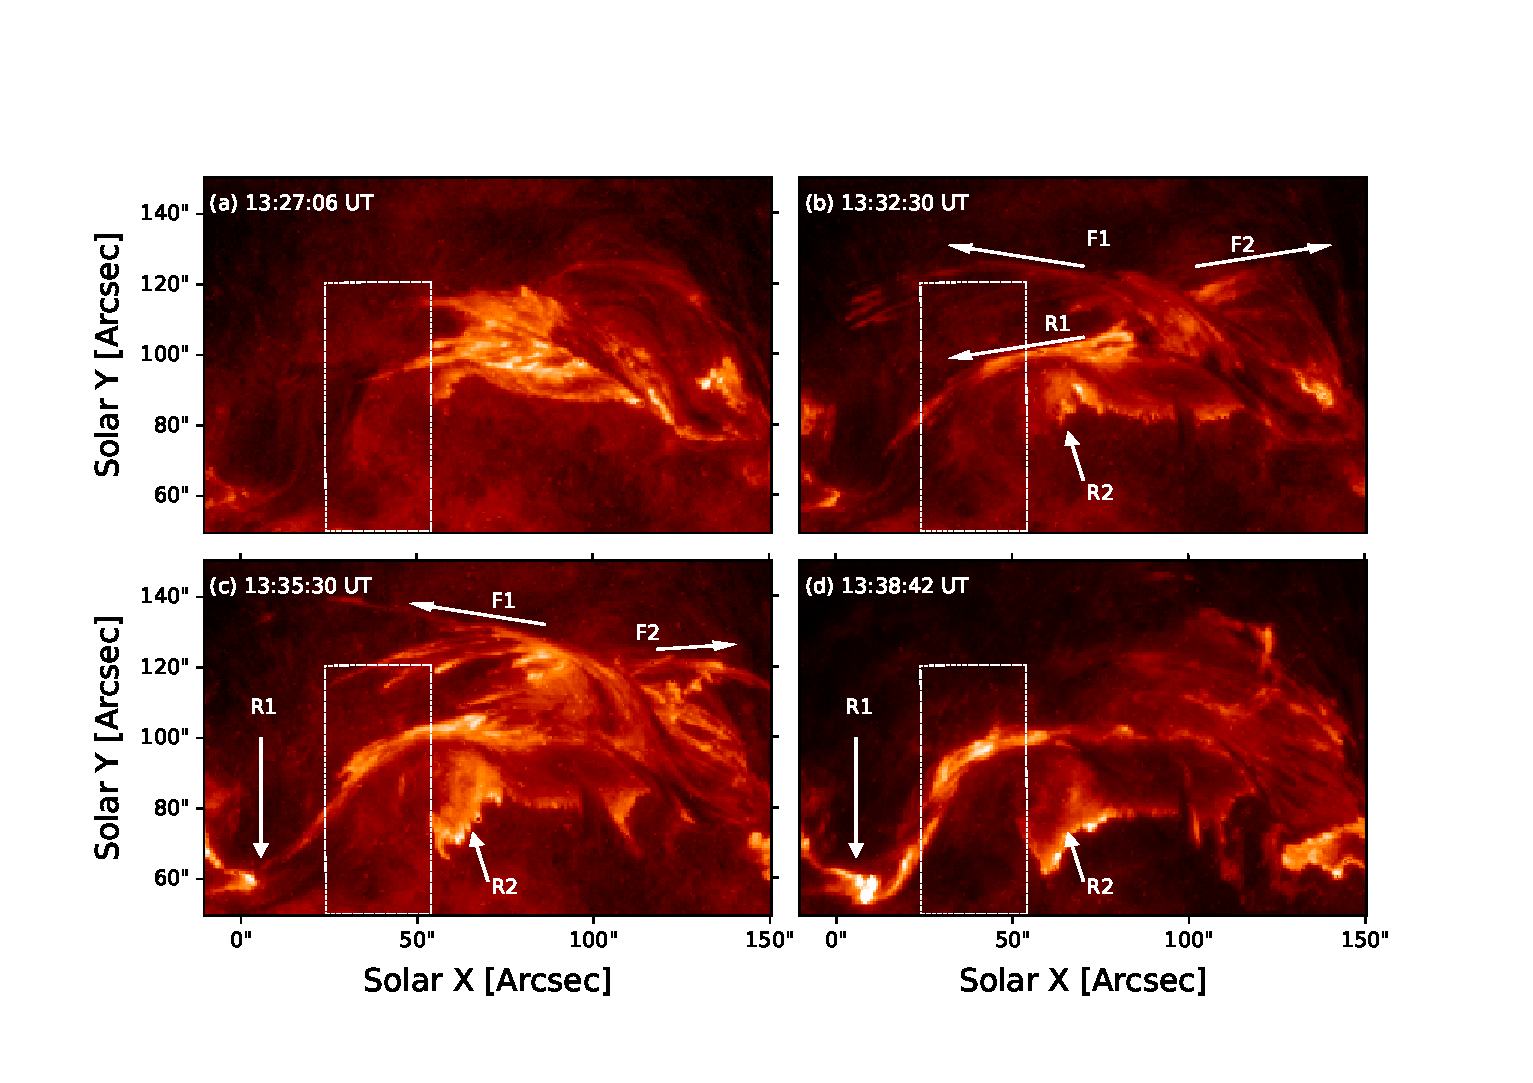
\includegraphics[width=\textwidth]{Figures/nov_flare_304_aa_evolv.eps}
    \end{center}
    \caption{Sequence of AIA 304~{\AA}~images for the Nov 4th, 2015 flare. The white dotted box shows the portion of the IRIS raster FOV which scanned the ribbons. In panels b (c) F1 and F2 are the filament material, which move away from each other as the flare progresses. R1 and R2 in b (c,d) show the primary ribbons which move through the IRIS raster FOV. An animation of this image sequence is available in \cite{roy24}.}
    \label{flare_m_ev}
\end{figure*}
%%%--------------

Fig.\ref{flare_m_aia} presents the same region as depicted in Fig.\ref{flare_m_ev} across the six coronal channels (i.e., 94, 131, 171, 193, 211, 335~{\AA}) of SDO/AIA, recorded at the peak (top two rows) and during the decline phase (bottom two rows) of the flare. Post-eruption arcades \citep[][]{TriBC_2004} are clearly observable in all the channels, displaying slightly varied morphologies. These arcades contain evaporated thermal plasma and exhibit loop top brightening, likely due to colliding evaporation flows \citep[see, e.g.,][]{sharma16, patsourakos04}.

%%%--------------
\begin{figure*}[ht!]
    \begin{center}
        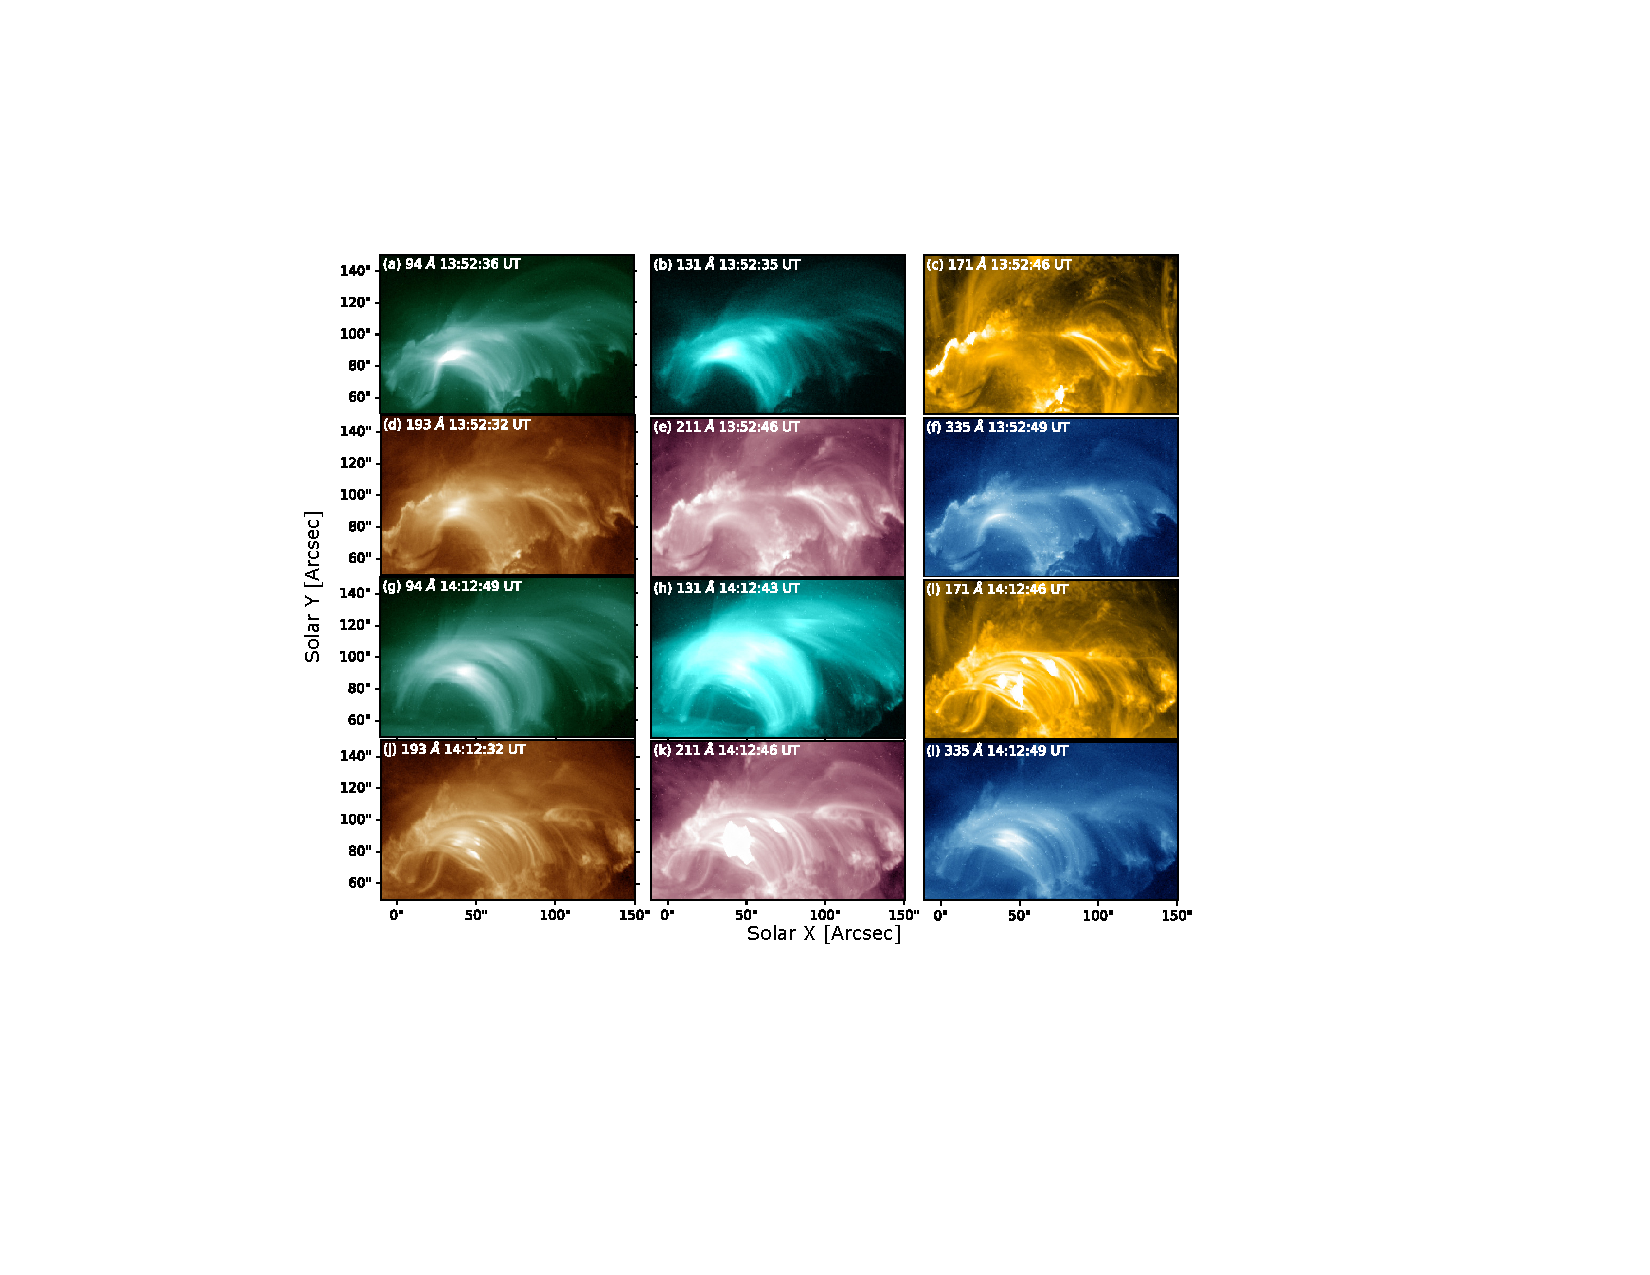
\includegraphics[trim={4.5cm 5.5cm 6cm 4cm},clip,width=\textwidth]{Figures/nov_flare_aia_waves_2.pdf}
    \end{center}
    \caption{The Nov 4th, 2015 flare in the six Coronal channels of the SDO/AIA at the soft X-ray peak (panels (a)-(f)) and during the decline phase (panels (g)-(l)) of the flare.}
    \label{flare_m_aia}
\end{figure*}
%%%--------------

We begin by aligning the HMI observations with the IRIS observations using the 1600~{\AA} data recorded by AIA. Given that the observation involves an active region undergoing flaring, the magnetic field may also be rapidly changing \citep{wang02,dandan16,spirock02}. Therefore, we utilize a series of co-aligned full-disk maps from AIA and HMI to derive a rastered line-of-sight (LOS) map of magnetic flux density that precisely corresponds to the location and time of IRIS rasters. This procedure is outlined below.

Initially, we align the AIA 1600~{\AA} observation with the HMI observation closest in time to the IRIS SJI (Slit-Jaw Imager) and raster observations. Using the `aia\_prep' tool available in the \textit{sswidl} distribution, we process the level 1 images to perform image registration and align AIA and HMI observations. Subsequently, we calculate the shift between AIA 1600~{\AA} and the SJI 1400~{\AA}. Using these calculated offsets, we co-align the magnetograms with the IRIS SJI 1400~{\AA} observations, given that the AIA 1600~{\AA} observation was already aligned with the HMI observations. We typically observe an offset of approximately $\sim$ 1.5\arcsec~between HMI and IRIS. These co-aligned HMI maps are then utilized to derive the rastered magnetograms, which can be directly compared with IRIS raster observations.

%%%%-------------------------
\begin{figure}[ht!]
\centering  
\vspace{10cm}
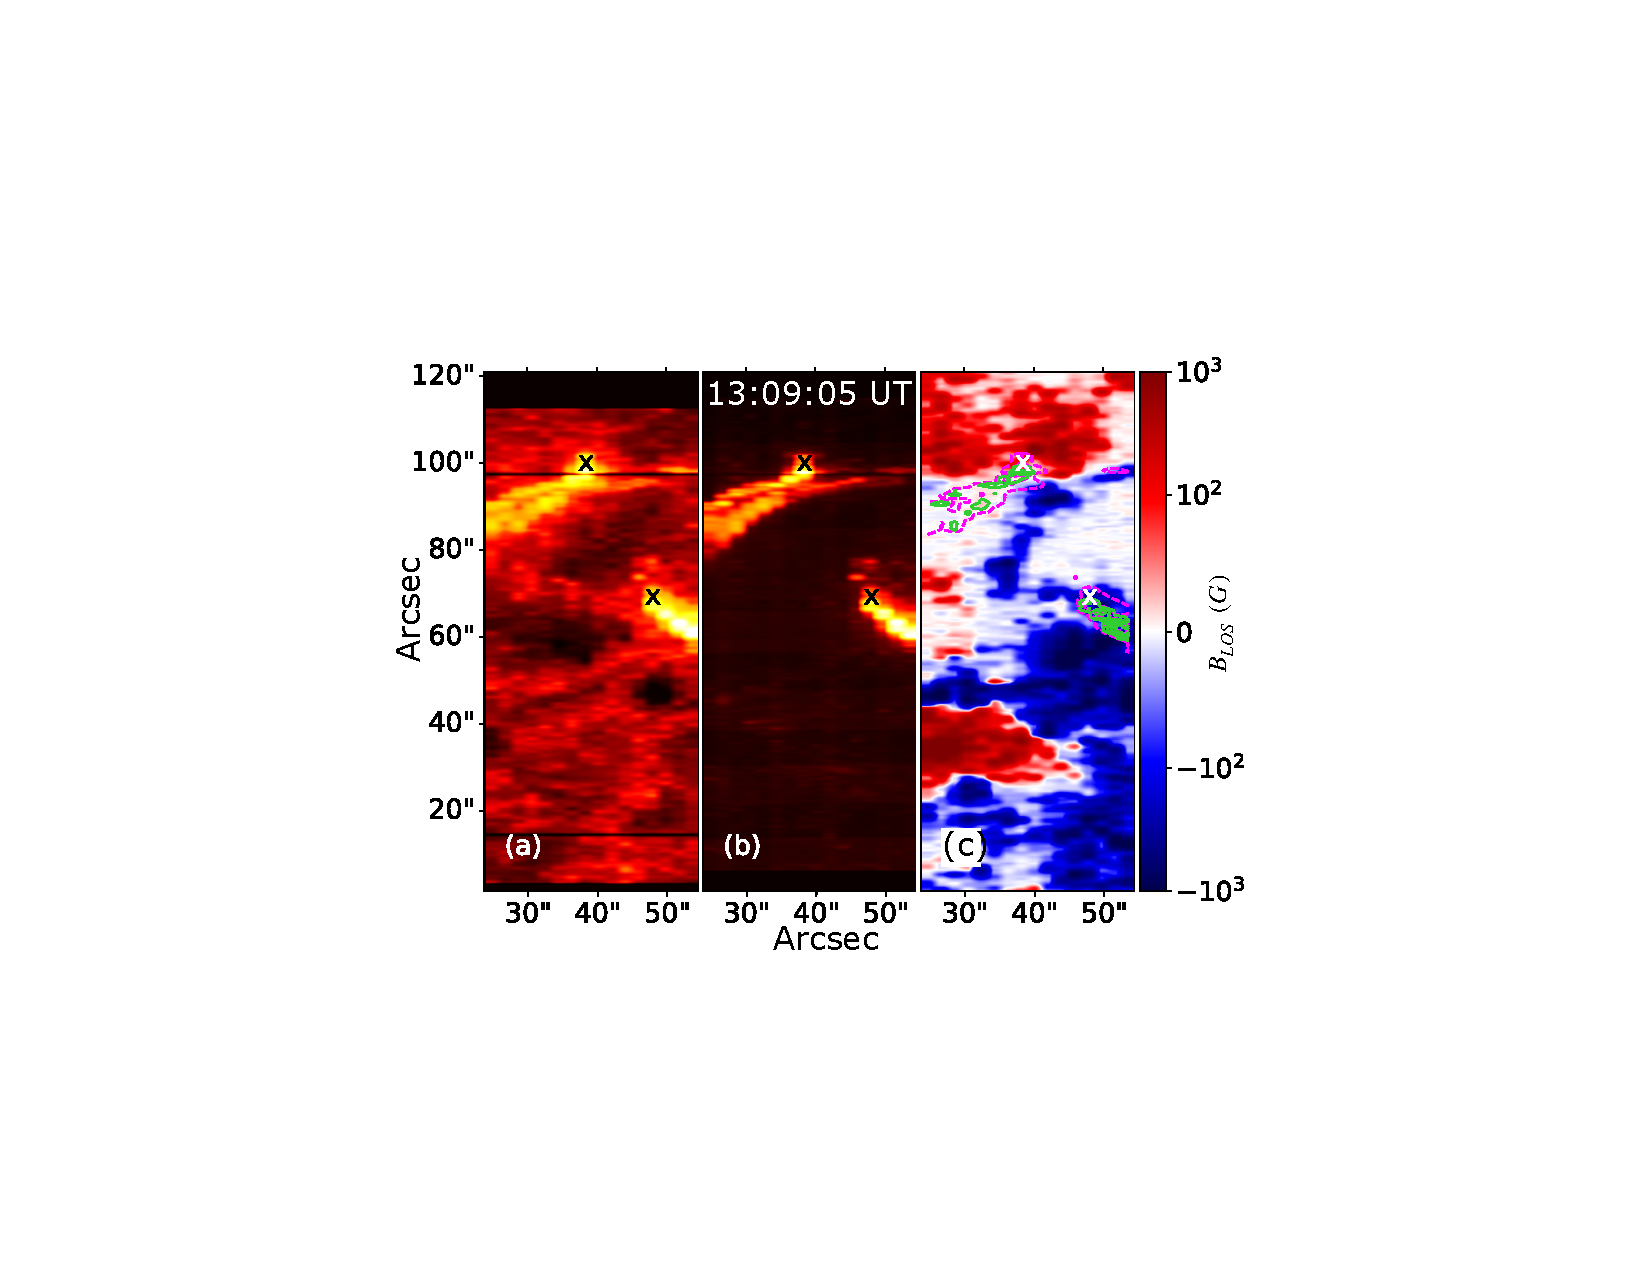
\includegraphics[trim={7cm 5cm 6cm 15cm},width=0.7\textwidth]{Figures/m_flare_iris.pdf}
\caption{Obtained images in  \ion{Mg}{2} h (panel a) and k (panel b) and corresponding co-aligned and artificially rastered HMI LOS magnetic field map (panel c) for the M3.7 flare observed on November 4th, 2015. The magenta and lime green contours on panel c show the contours of  \ion{Mg}{2}~h (panel a) and k (panel b) intensity.} \label{fig:aligned_raster}
\end{figure}
%%%%-------------------------

For analyzing the properties of the  \ion{Mg}{2} lines, we fit a double Gaussian profile to both the k and h lines with a linear background symmetric about the line core. If excess emission is detected compared to the fitted background and line profile for wavelengths lower than 2792~{\AA} and in-between 2798~{\AA} to 2800~{\AA}, we infer the presence of  \ion{Mg}{2} triplets in emission. A single Gaussian profile is fitted to the excess emission. It's important to note that this approach may overlook the triplets unless the emission is sufficiently strong. However, this method serves our purpose since our primary objective is to characterize the  \ion{Mg}{2} k and h line profiles.

Additionally, we exclude any pixels showing saturation in either of the lines. The uncertainty of the observed intensities is measured in DN (Data Numbers) using the method outlined in \S2.1 of \cite{kerr15} and subsequently applied in the fitting procedure. The uncertainties of the fitted Gaussian profiles are incorporated while integrating the profile to obtain the uncertainty of the line intensities.

%%%%%%%%%%%
\begin{figure*}[ht!]
    \centering
    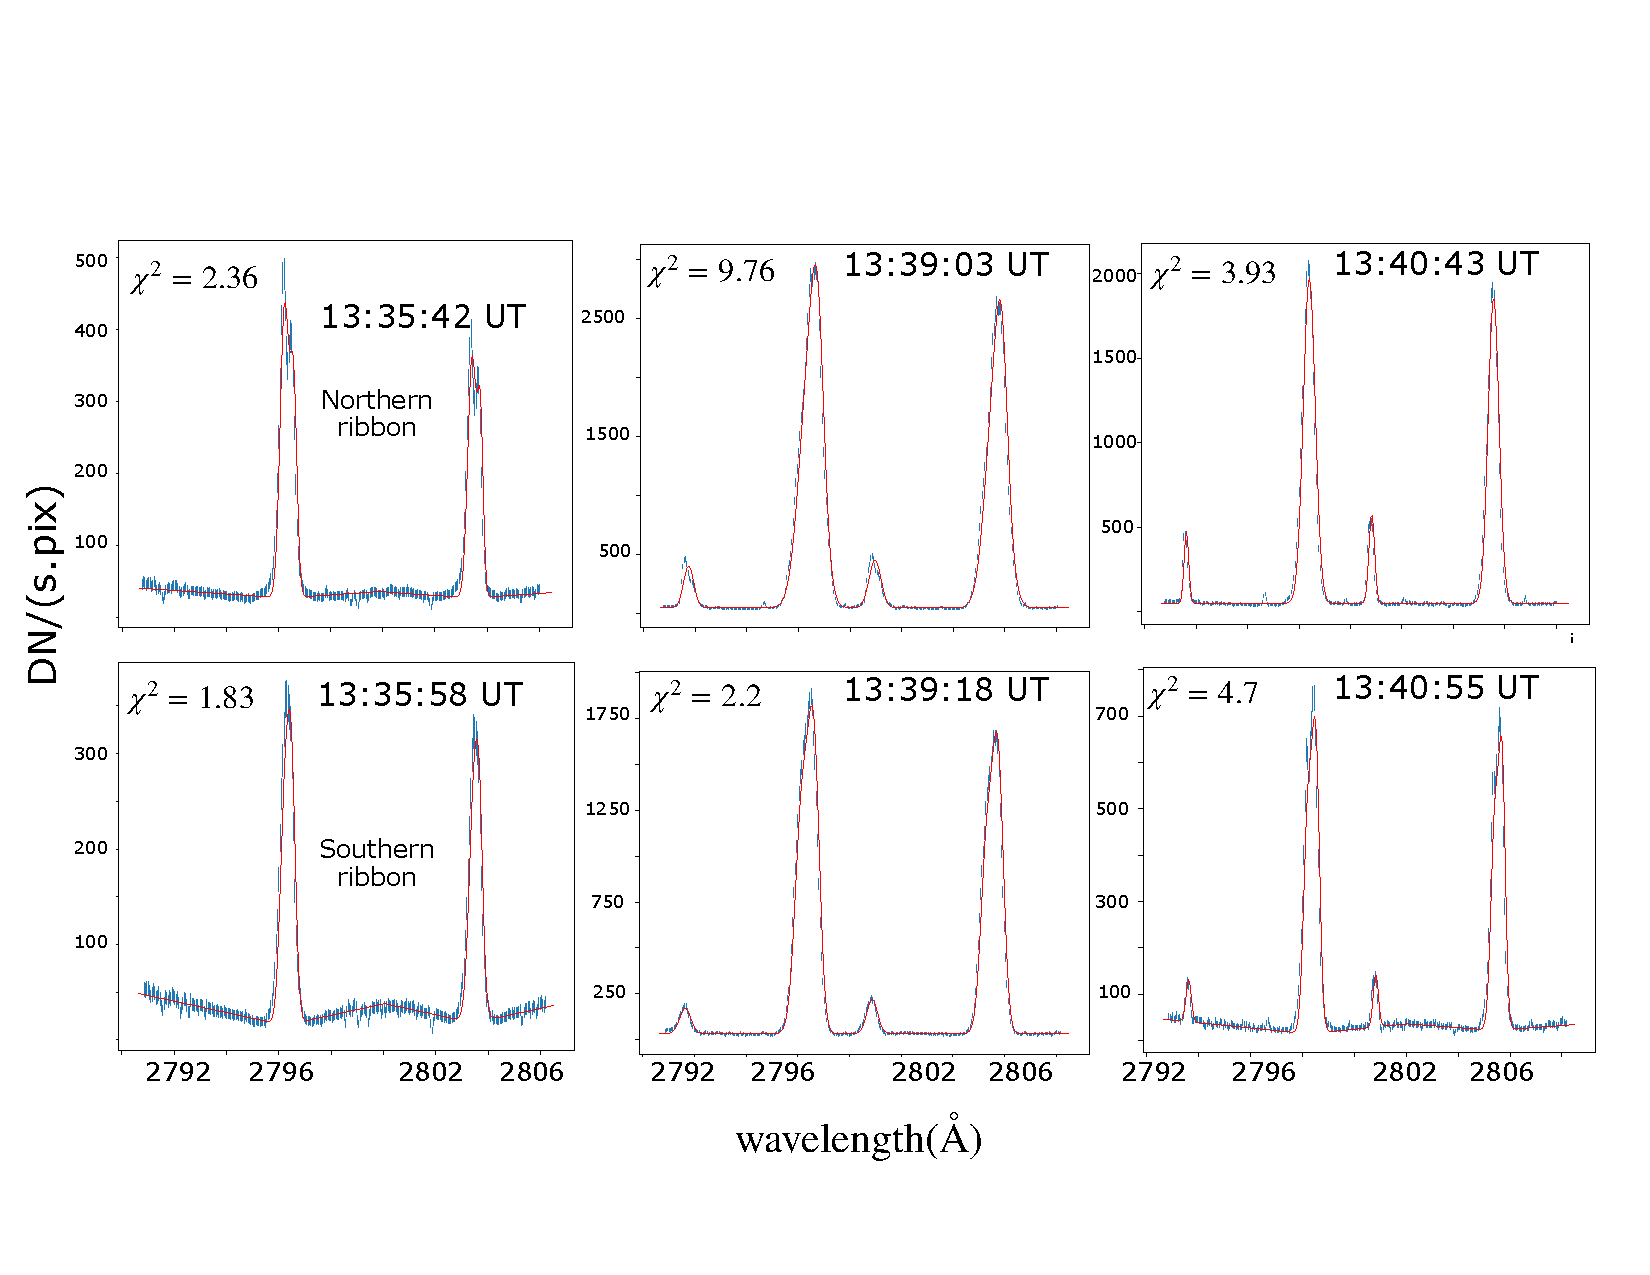
\includegraphics[trim={0cm 3cm 0.5cm 3cm},clip,width=\textwidth]{Figures/pix_fit.pdf}
    \caption{Fit of the  \ion{Mg}{2} window for the pixel marked in northern ribbon (southern ribbon) in Fig.~\ref{fig:aligned_raster} in top panel (bottom panel) from various times during the evolution of the flare. }
    \label{fig:pix_fit_ribbon}
\end{figure*}
%%%%%%%%%%%

%%%%-------------------------
\begin{figure}[ht!]
\centering  
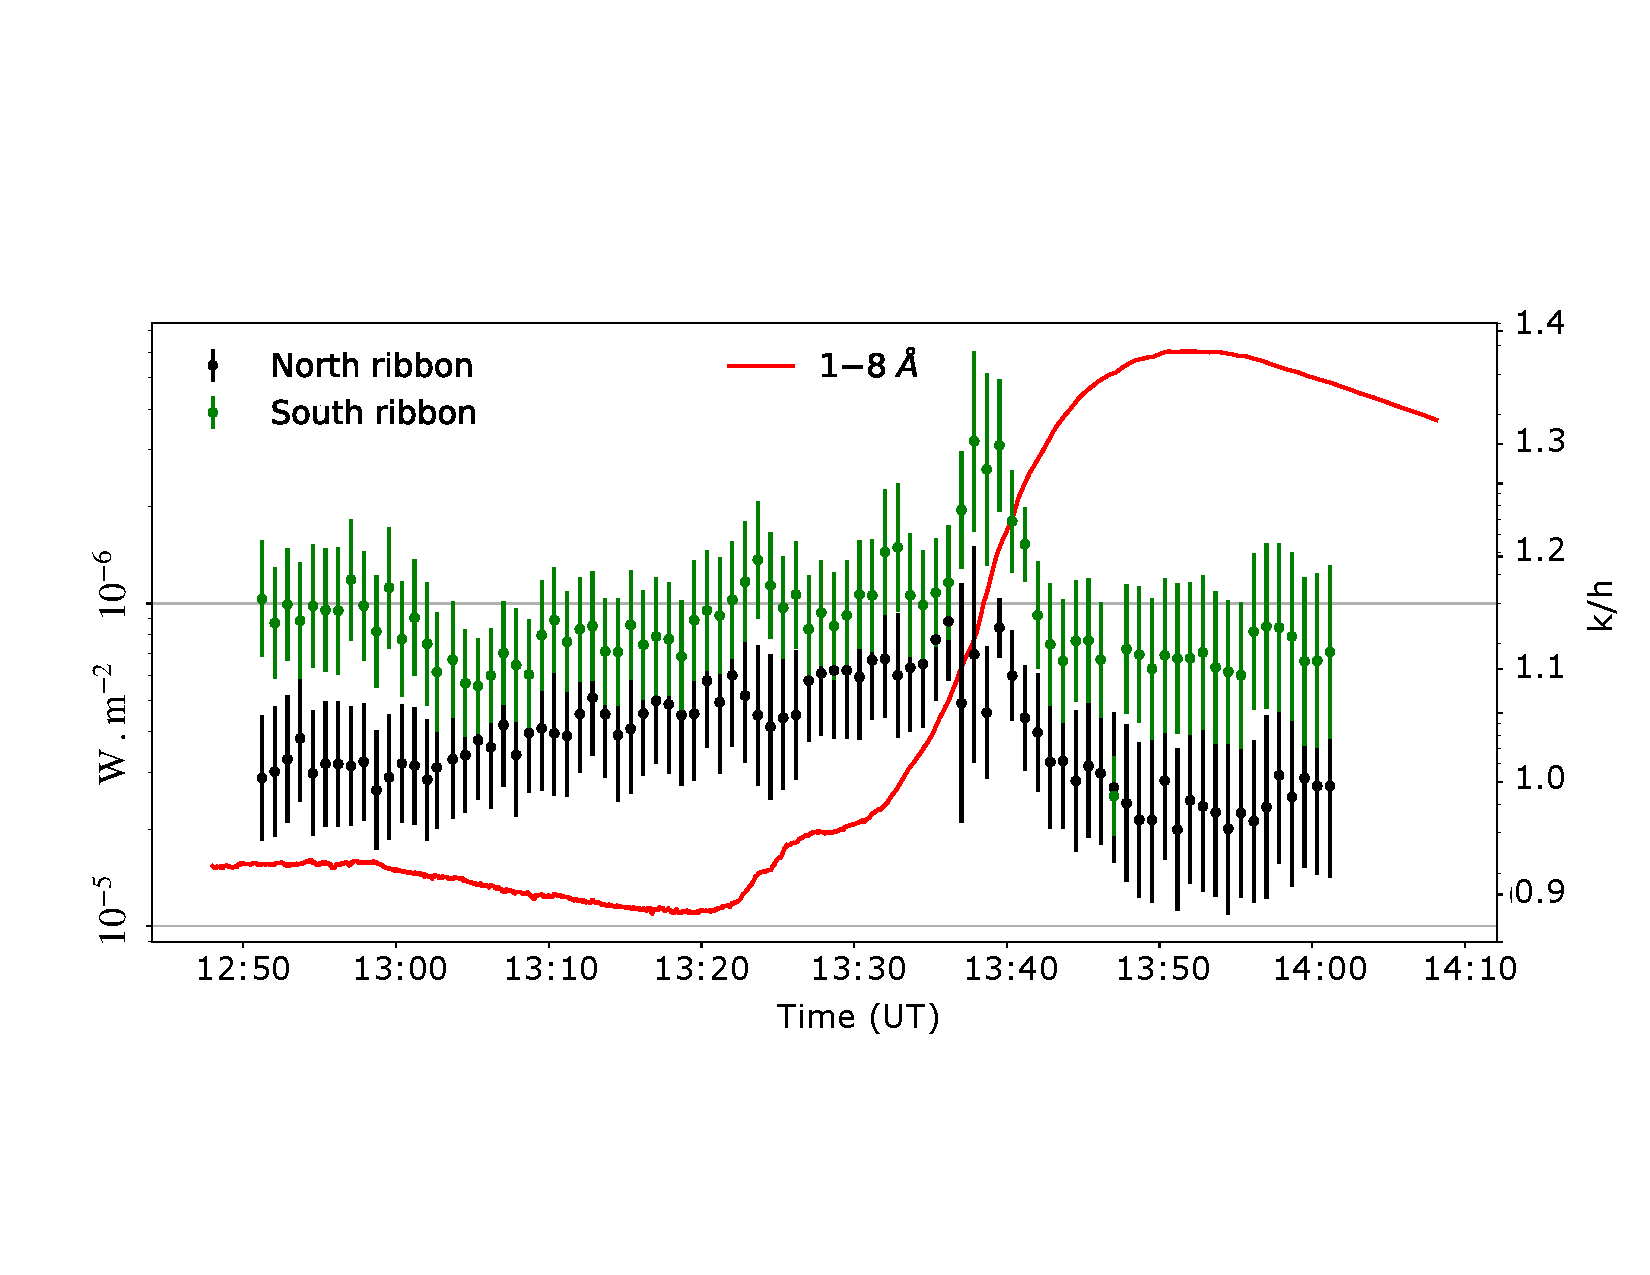
\includegraphics[trim={1.5cm 4cm 0.5cm 4cm},clip,width=0.8\textwidth]{Figures/m_flare_iris_pt2.pdf}
\caption{The 1{--}8~{\AA} GOES light curve of the flare over-plotted with the time variation of  \ion{Mg}{2} k/h line intensity ratio for the northern (black) and southern (green) asterisks marked in panels a, b \& c.}
\label{fig:aligned_iris_ratio}
\end{figure}
%%%%-------------------------

In Figure~\ref{fig:aligned_raster}, we present intensity maps obtained in  \ion{Mg}{2} h \& k (panels a \& b) alongside the rastered line-of-sight (LOS) magnetic field map in panel (c). The dashed magenta and solid green contours on the magnetic field maps represent the intensity from panels a and b, respectively. To investigate the  \ion{Mg}{2} k to h intensity line ratios over time, we selected two pixels—one in the northern ribbon and another in the southern ribbon, as indicated by crosses. Fig.~\ref{fig:pix_fit_ribbon} displays the spectra overlaid with fits for the two pixels taken in the northern ribbon (top panel) and southern ribbon (bottom panel) obtained at different times.

We illustrate the  \ion{Mg}{2} k to h line intensity ratio derived from the two locations in the northern (black) and southern ribbons (green) in Fig.\ref{fig:aligned_iris_ratio}. Additionally, we overlay the GOES light curve of the flare obtained in 1.0{--}8.0{\AA} (red solid line). Our observations indicate that the intensity ratios exhibit a slightly increasing trend, albeit within the margin of errors, during the early phase of the flare. The ratio demonstrates a distinct peak around the midpoint of the impulsive phase, lasting for a very brief duration of approximately 150 seconds, before beginning to decrease. It's worth emphasizing that the pixel-by-pixel fitting of the  \ion{Mg}{2} h \& k line profiles provided a sufficient signature of the time evolution of the k/h line intensity ratio during the flare.

%%%%%%%--------%%%%%%%%%%%
\subsection{Investigating the dependence on the local magnetic field in the  \ion{Mg}{2} lines}
%%%%%%%---------%%%%%%%%%%

To explore the time evolution of the intensity ratio and its potential relationship with the photospheric magnetic field, we binned the spectra into various magnetic field bins from different flaring pixels. We selected the flaring pixels based on an intensity threshold relative to the peak intensity observed in IRIS rasters. A double Gaussian fit with a constant background was performed in a smaller wavelength window for both the  \ion{Mg}{2} h and k lines separately. This step was essentially carried out to mitigate the effects of the background and potential contributions from other spectral features.

Fig.~\ref{fig:fit_pix_fov} displays the  \ion{Mg}{2} k line profiles obtained at different times and averaged over different magnetic field bins. Each plot denotes the observation time and the magnetic field strength over which the spectra were averaged and fitted with a double Gaussian. Line intensities were computed by integrating the fitted Gaussian.

In Fig.~\ref{fig:optical_depth_m}, we present the k to h intensity ratios obtained in various bins of magnetic flux density at different times corresponding to different flare phases. The curve corresponding to 13:07:05 UT (red) represents the pre-flare phase, where the ratio is approximately 1.2. The ratio shows an increase during the impulsive phase, i.e., the curves corresponding to 13:23:44 UT (blue dotted) and 13:32:04 UT (green dashed). The ratio measured at 13:41:11 UT (magenta dashed), which is closest to the UV peak of the flare, exhibits the largest value across all magnetic field bins. Subsequently, during the decline phase, the ratio measured at 13:57:23 UT (black solid) falls below the values observed during the pre-flare phase. Additionally, it's noteworthy that there are no significant differences among the k to h ratios obtained in different bins of magnetic flux density at all times (including pre-flare, impulsive, peak, and decline phases) of the flare.

%%%%-----------------------
\begin{figure*}[ht!]
    \begin{center}
    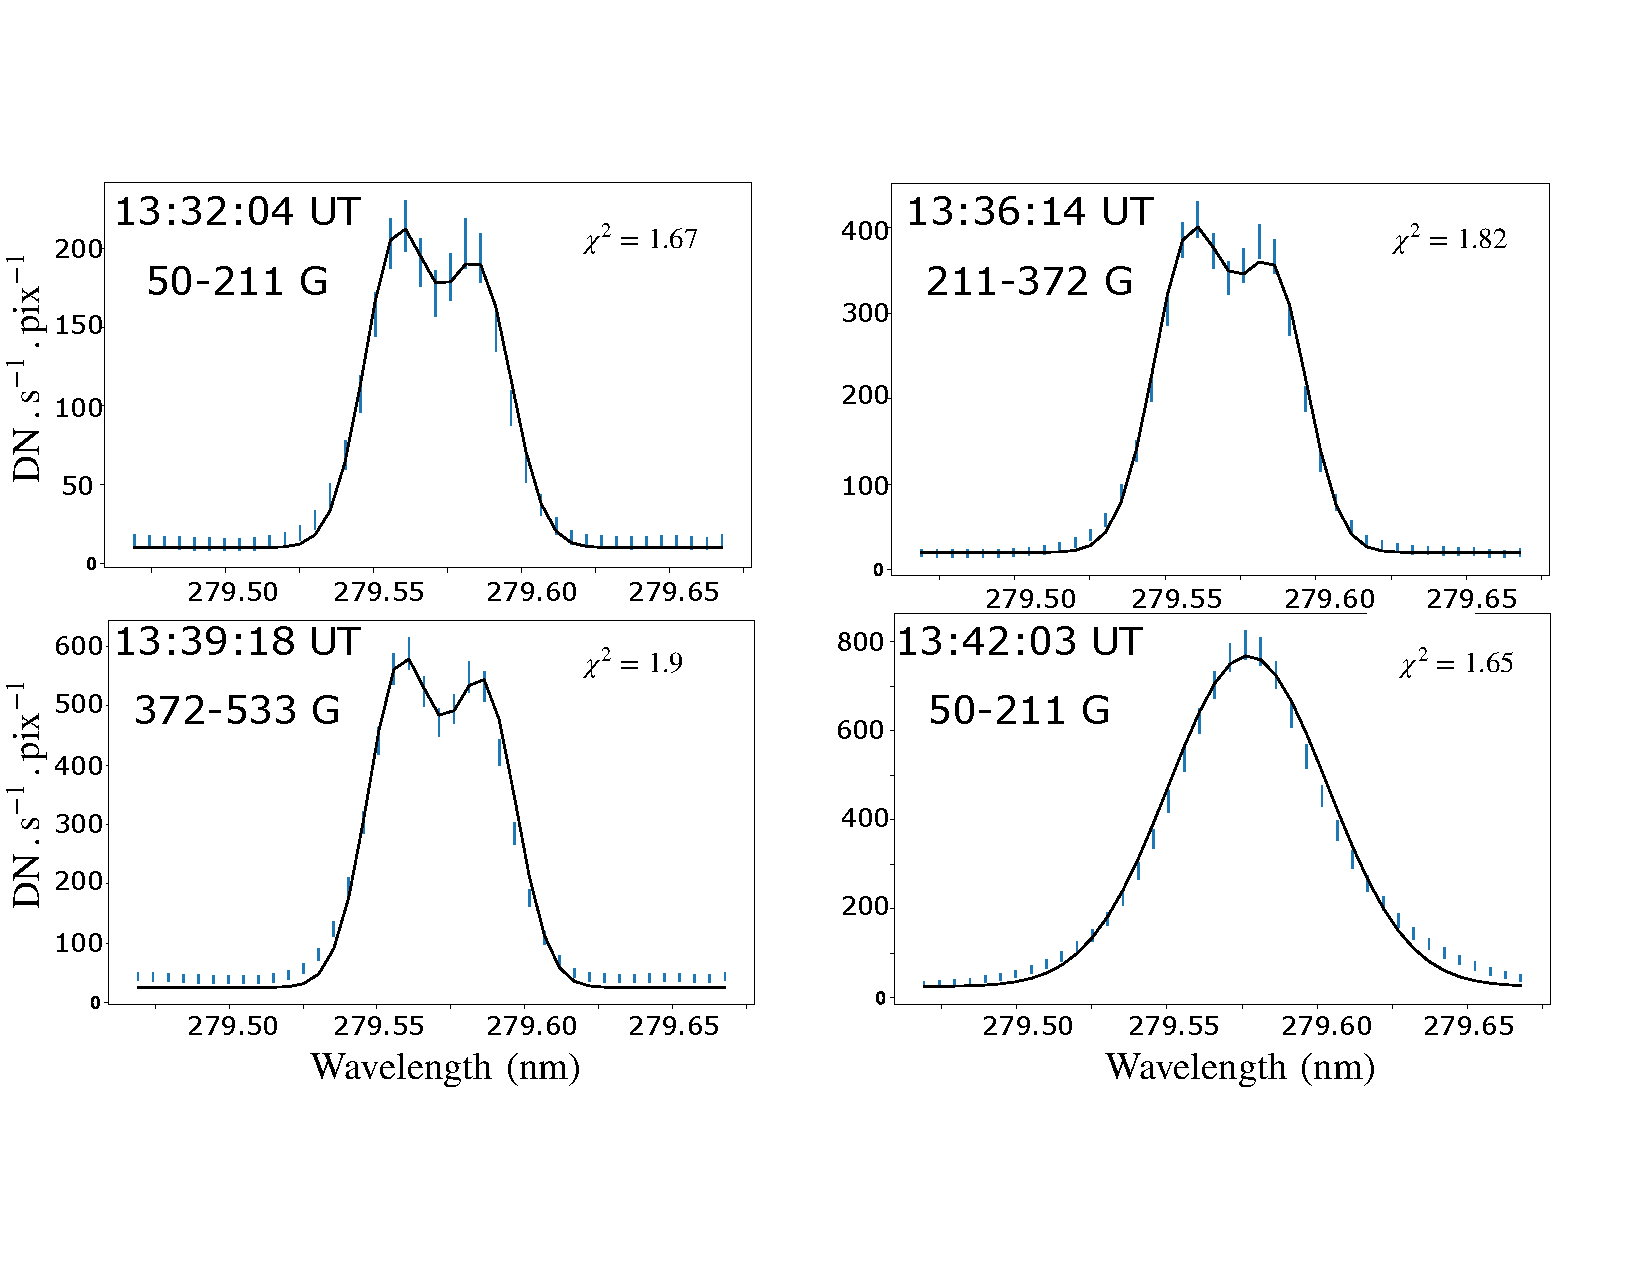
\includegraphics[trim={0cm 3cm 0cm 3cm},clip,width=\textwidth]{Figures/binned_fit_fov.pdf}
    \end{center}
    \caption{Fitted line profiles for the binned spectra for various magnetic field strengths from various times.}
    \label{fig:fit_pix_fov}
\end{figure*}
%%%%----------------------- 

%%----------------------------------------------------------------------------
\begin{figure}[ht!]
    \centering
    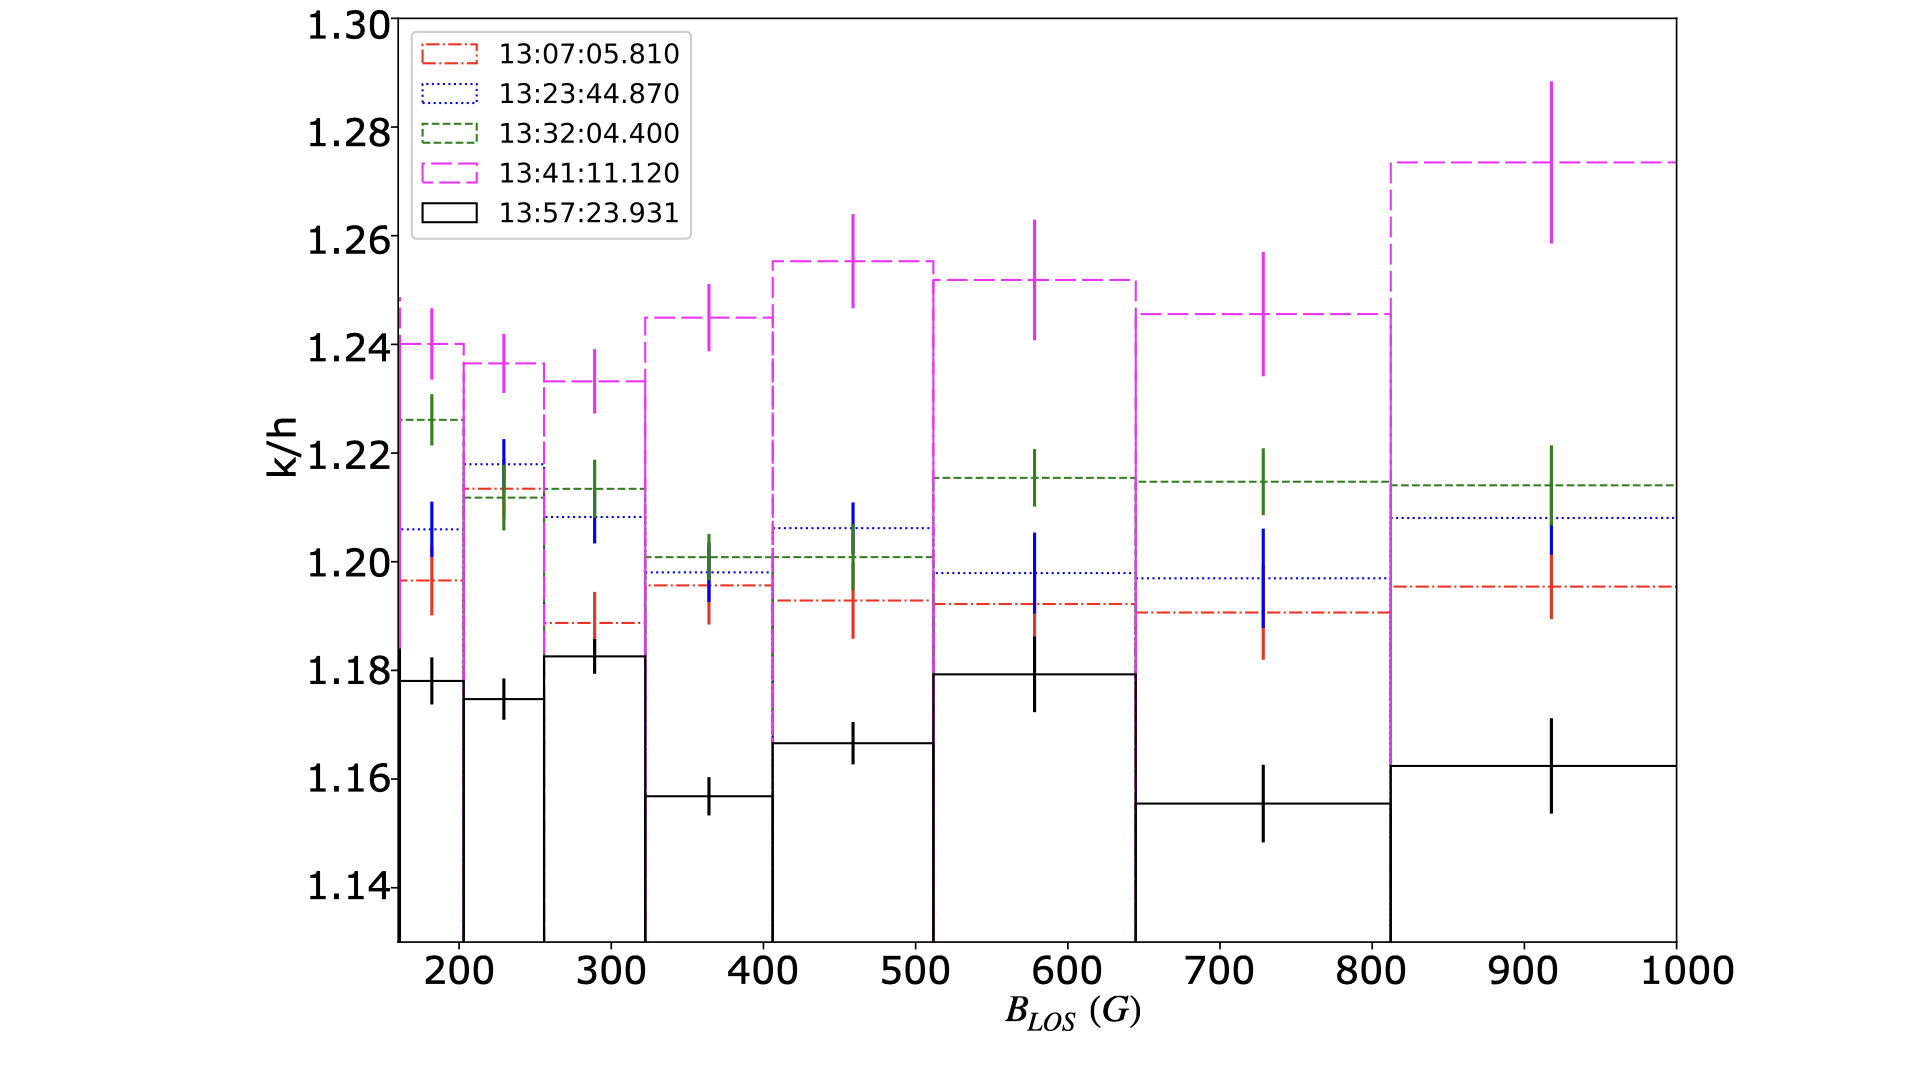
\includegraphics[trim={8cm 1cm 2cm 0.2cm},clip,width=0.9\textwidth]{Figures/Flare-m-optical-depth-2.jpeg}
    \caption{ \ion{Mg}{2} k to h line intensity ratio for various magnetic flux density bins at various time steps during the evolution of the flare.}
    \label{fig:optical_depth_m}
\end{figure}
%%----------------------------------------------------------------------------

To explore further, we study the evolution of k to h intensity ratio as a function of time during the flare. In Fig.~\ref{fig:optical_dep_ev_m}, we plot the time evolution of the k to h line intensity ratio averaged within the bins of different magnetic flux densities as a function of time. For better visibility the 20.9{--}184.4 G and 348.9{--}513.3 G points are offset by 30s and -30s, respectively. We also plot the GOES 1{--}8~{\AA} light curve with the red solid line. These plots conspicuously reveal that the intensity ratios rise sharply during the impulsive phase, from $\sim$ 1.20 to $\sim$ 1.28 right before the soft X-ray flux peaks as seen from GOES, and decreases very rapidly thereafter, to lower than pre-flare values $\sim$ 1.12. The typical uncertainty value for the line intensity ratio is $\sim$ 0.02. We further note that the evolution of the  \ion{Mg}{2} k to h intensity ratio is remarkably similar across various strengths of magnetic flux densities.

%%%----------------------------------------------
\begin{figure*}[ht!]
    \centering
    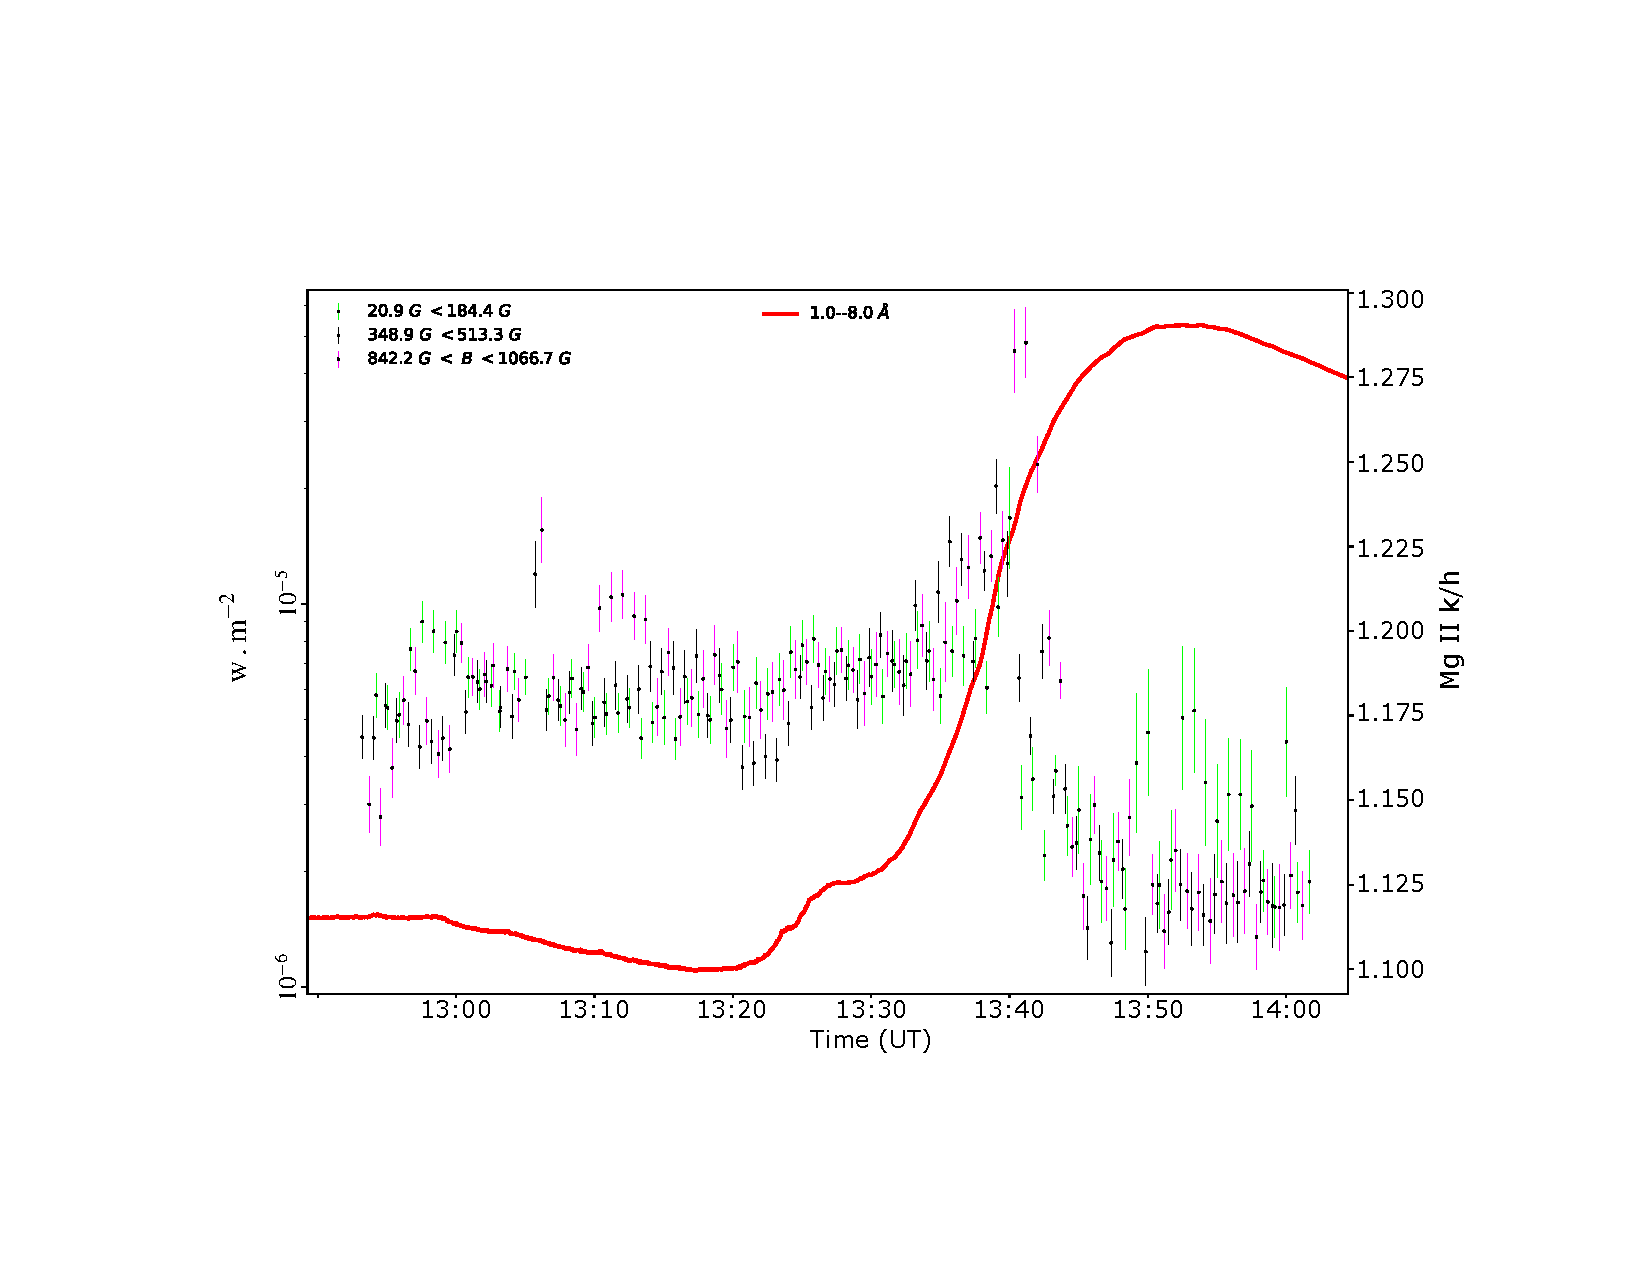
\includegraphics[trim={3cm 3cm 2cm 4cm},clip,width=\textwidth]{Figures/Nov-11-2015-optical-dep-ev-5.pdf}
    \caption{Time evolution of the  \ion{Mg}{2} k to h line intensity ratio obtained from averaged spectrum over the corresponding magnetic flux bin as labeled for the Nov 4, 2015 flare. For better visibility, the 20.9{--}184.4 G and 348.9{--}513.3 G points are offset by 30s and -30s respectively. Over-plotted red solid line displays the 1{--}8~{\AA} GOES X-ray light curve.}
    \label{fig:optical_dep_ev_m}
\end{figure*}
%%%----------------------------------------------

%%%----------------------------------------------
\subsection{X1.6 Flare Observed on Oct 22, 2014}
%%%----------------------------------------------

An X~1.6 flare occurred on October 22, 2014, observed in AR 12192. The flare commenced at 14:02 UT and peaked at 14:28 UT as observed by GOES. Fig.\ref{flare2}(a) illustrates the GOES flux plot of the flare in the 0.5{--}4~{\AA} range (blue) and the 1.0{--}8.0~{\AA} range (red). Figs.\ref{flare2}(b) \& (c) display an AIA 1600{\AA} image and the line-of-sight (LOS) magnetic flux density map obtained from HMI, respectively. The overlaid boxes in panels (b) and (c) indicate the IRIS SJI (Slit-Jaw Imager) field of view (FOV). IRIS observed this flare with a large 8-step coarse raster covering a FOV of [14\arcsec,174\arcsec]. It's worth noting that the IRIS SJI FOV and the slit direction were rotated by approximately 45$^\circ$ relative to the center of the HMI observation.

%%--------------------------------------------------
\begin{figure}[ht!]
    \centering
\hspace*{-.5in}
\includegraphics[width=\textwidth,trim={7cm 5cm 7.7cm 6cm},clip]{Figures/Flare_X_oct22_2014_2.eps}
\caption{The X class flare observed on October 22, 2014. Panel a: GOES flux plot in 0.5{--}4~{\AA} (blue) and 1.0{--}8.0~{\AA} (red). Panel b: AIA 1600~{\AA} image taken at the peak of the flare. Arrows locate the primary and secondary ribbons. Panel c: LOS magnetic flux density map obtained from HMI at the peak of the flare. The over-plotted white (black) box in panel b (c) represents the IRIS SJI FOV, and white dot-dashed (dashed) box in panels b (c) represents the IRIS Raster FOV.}\label{flare2}
\end{figure}
%%--------------------------------------------------

The flare manifests two ribbons in AIA 1600 {\AA}, as indicated by the arrows. The eastern ribbon extends around a negative field region and is entirely covered by the IRIS SJI FOV. Conversely, the western ribbon extends around a positive field region, with only a portion of it covered by the IRIS SJI FOV, as depicted in panel (b). In Fig.~\ref{fig:align_raster_flare2}, we present intensity maps obtained in  \ion{Mg}{2} h \& k (panels a \& b) alongside the rastered line-of-sight (LOS) magnetic field map (panel c). The black \& green dashed contours in the LOS magnetic field map (panel c) indicate the intensity contours of  \ion{Mg}{2} h \& k (panels a \& b).

%%--------------------------------------------------
\begin{figure}[ht!]
    \centering
%    \hspace{2in}
    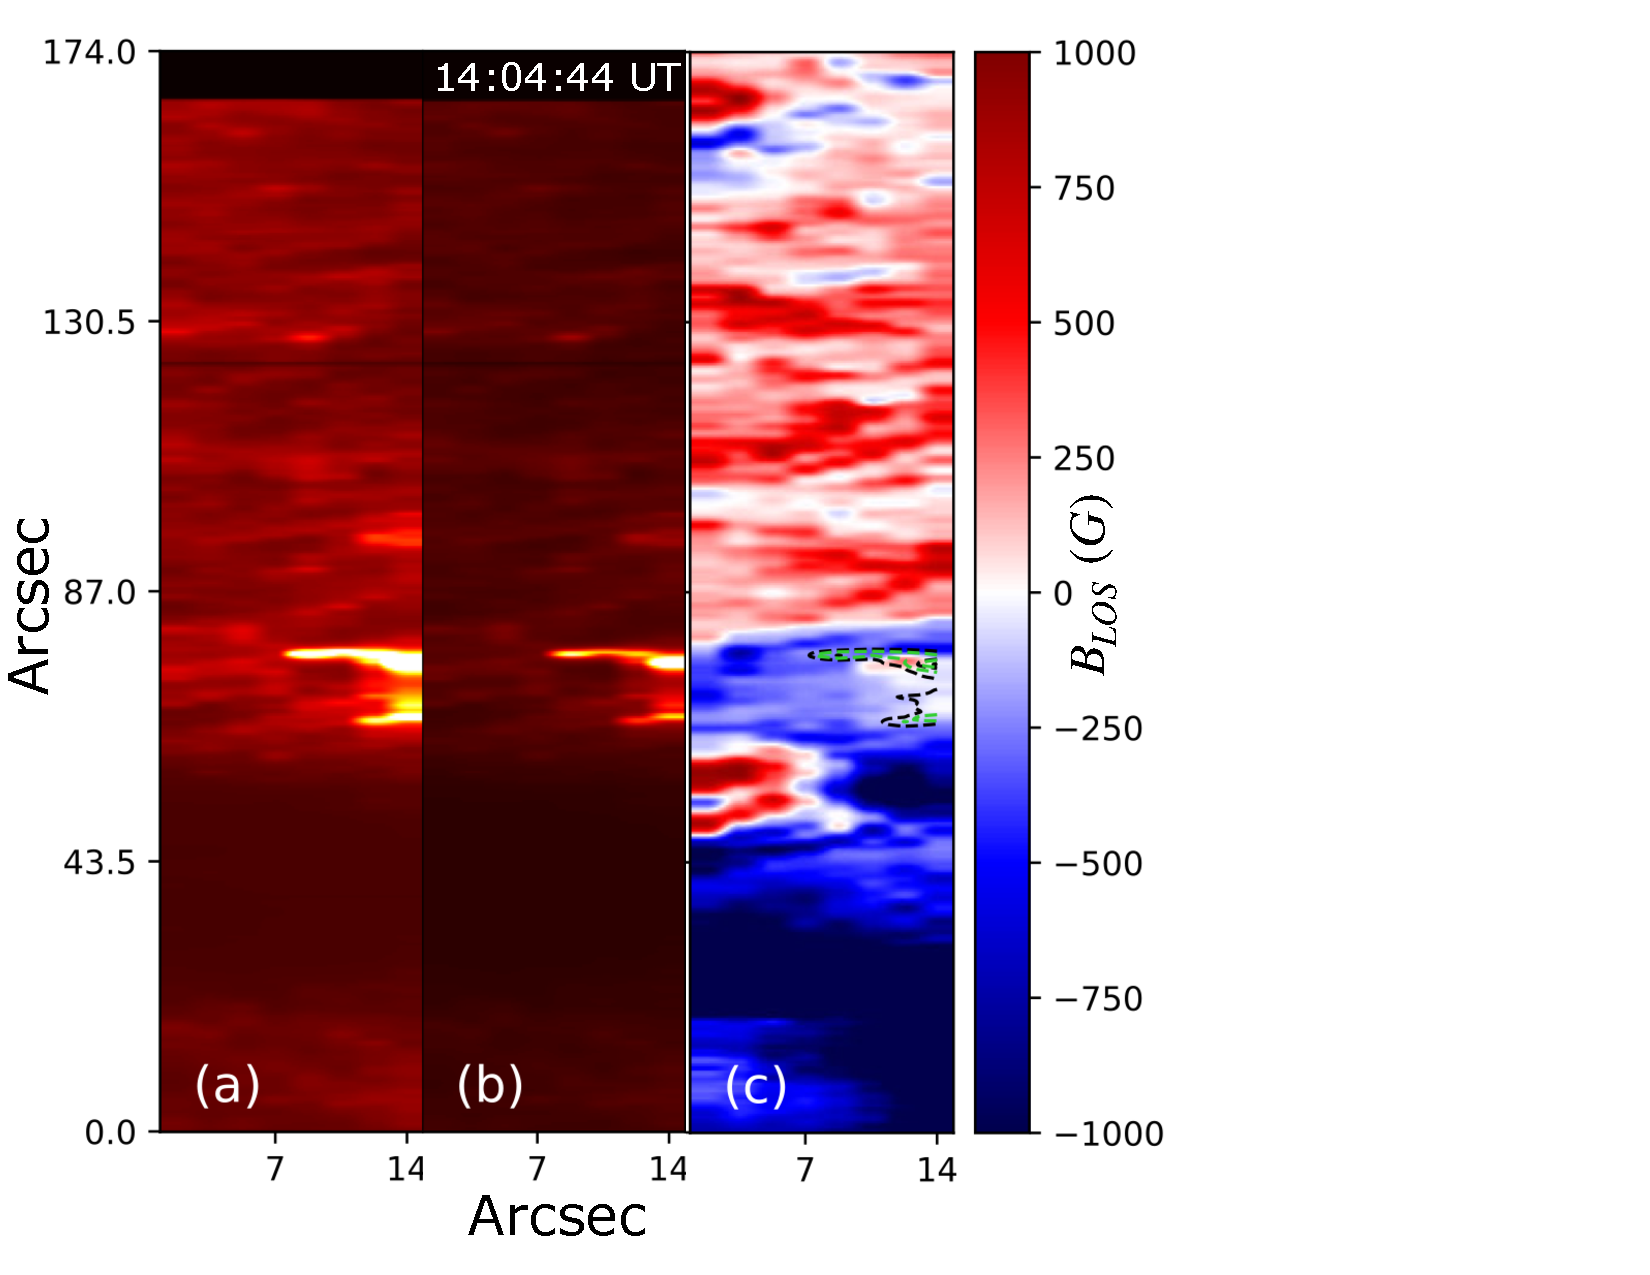
\includegraphics[trim={6cm 3cm 6cm 3cm},clip,width=0.45\textwidth]{Figures/contour_paper_plot_oct28.pdf}
    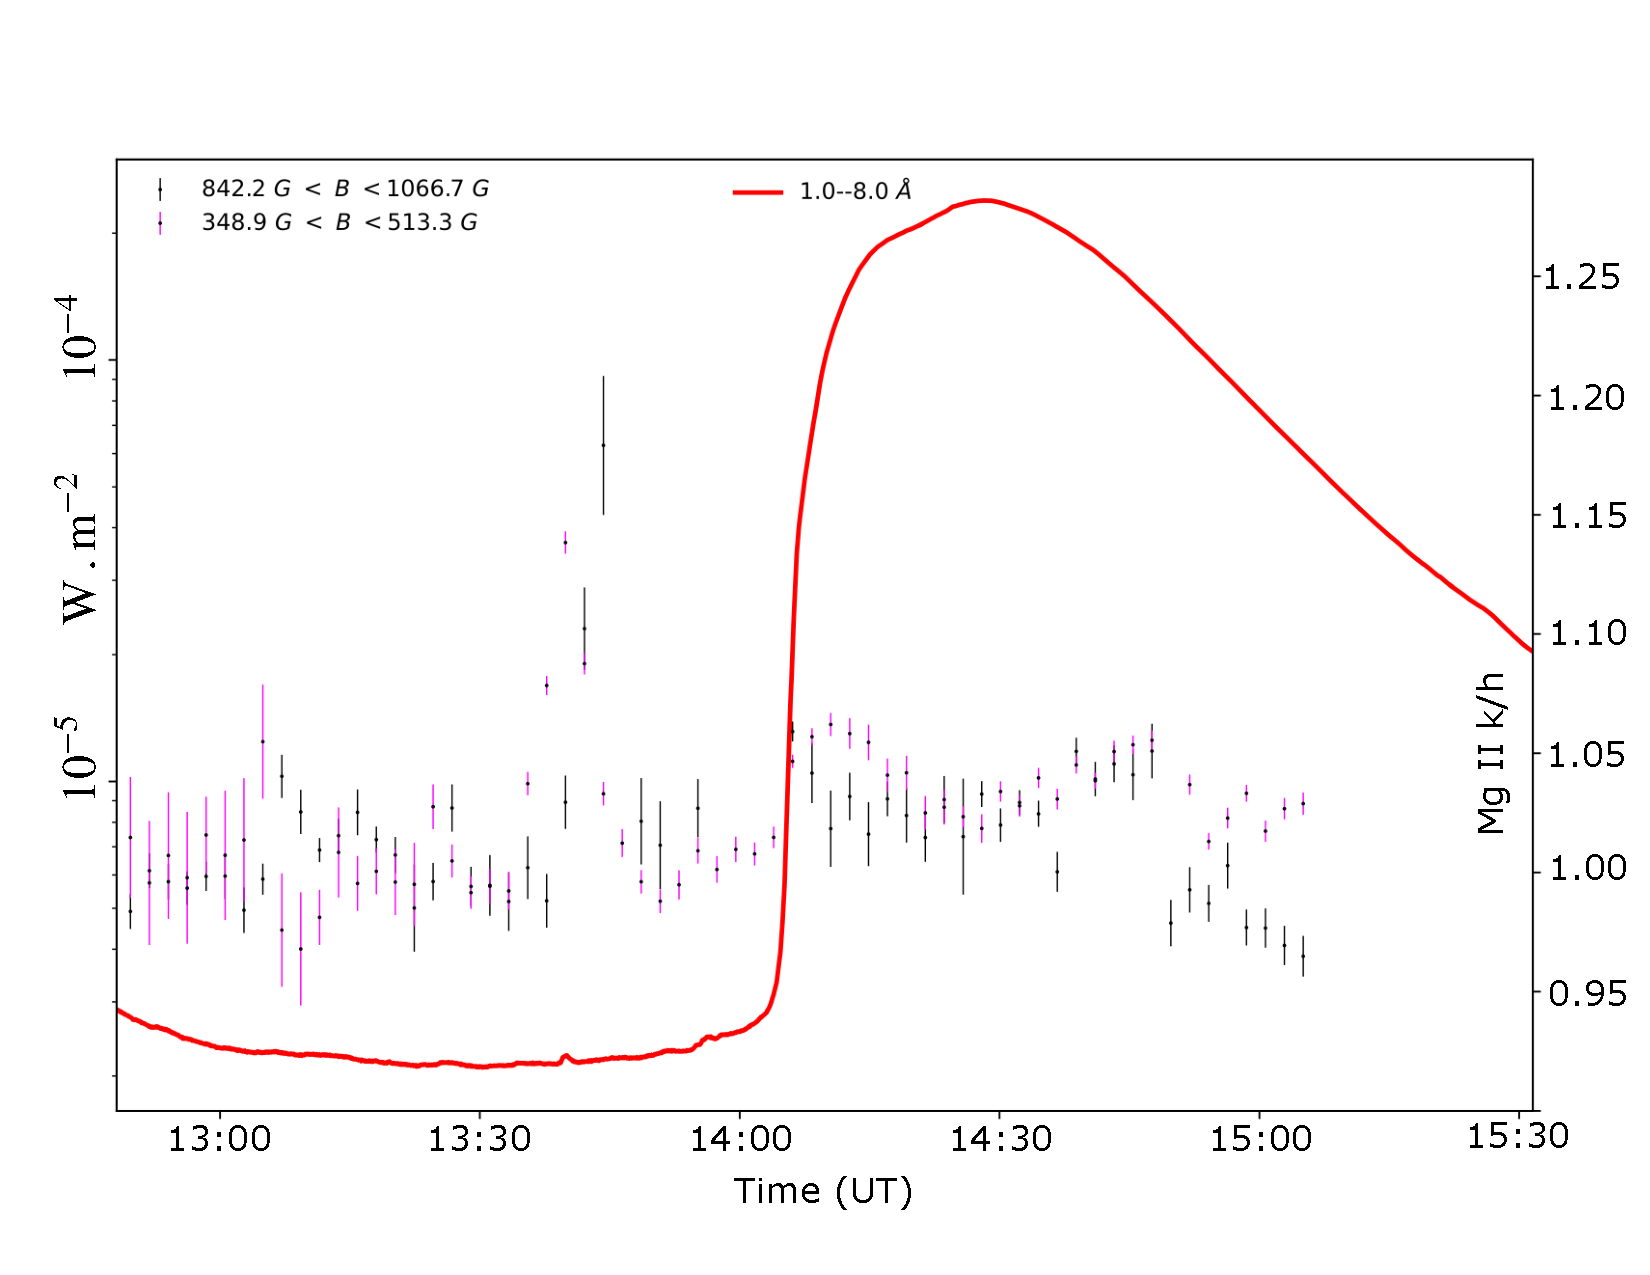
\includegraphics[trim={3cm 2cm 2cm 3cm},clip,width=0.45\textwidth]{Figures/Oct-22-2014-optical-dep-ev-2.pdf}
    \caption{Obtained intensity maps in  \ion{Mg}{2}~k (panel a) and h (panel b) lines at the peak of the flare. The rastrered HMI LOS magnetic field density map is shown in panel c. The black and lime green contours on panel c show the contours of  \ion{Mg}{2}~k (panel a) and h (panel b) intensity.}
\label{fig:align_raster_flare2}
\end{figure}
%%--------------------------------------------------

Similar to the M-class flare studied in the previous section, we derive the  \ion{Mg}{2} k to h line intensity ratio for various bins of the magnetic flux density within the flaring region and study their time evolution. In Fig.\ref{fig:align_raster_flare2} right panel, we plot the intensity ratio in black and magenta colors for two different magnetic field bins. In the same panel, we also overlay the 1{--}8~{\AA} GOES light curve (red solid line). We note that, unlike the M-class flare, we do not observe any noticeable change in the intensity ratio during the flare. There are approximately two to three data points showing an enhancement in the ratio, but these occur well before the onset of the flare.

%%%----------------------------------------------
\subsection{C3.5 Flare Observed on Feb 03, 2015}
%%%----------------------------------------------

On February 3, 2015, AR 12277 generated a C-class flare that peaked at 22:55 UT. Fig.\ref{flare3} depicts the GOES flux plot of the flare in the 0.5{--}4 {\AA} range (blue) and the 1.0{--}8.0 {\AA} range (red) in panel (a). Fig.\ref{flare3}(b) \& (c) displays an AIA 1600 {\AA} image and the line-of-sight (LOS) magnetic flux density map obtained from HMI, respectively, recorded near the peak of the flare.

The overlaid white (black) box in panel (b) ((c)) indicates the IRIS SJI (Slit-Jaw Imager) field of view (FOV). The over-plotted white dot-dashed (magenta dashed) box in panel (b) ((c)) indicates the IRIS raster FOV. IRIS observed this flare with a large dense 16-step raster with a FOV of 5"$\times$119" and a step size of 0.35\arcsec. The flare exhibits a double ribbon structure, with the east ribbon elongating earlier and merging into the west ribbon. The IRIS raster scans through the west edge of the west ribbon through its eruption and merging with the east ribbon. Fig.~\ref{fig:align_raster_flare3} displays the intensity maps obtained in  \ion{Mg}{2} h \& k (panels a \& b). The rastered LOS magnetic field map is shown in panel (c). The black \& green dashed contours in the LOS magnetic field map (panel c) depict the intensity contours of  \ion{Mg}{2} h \& k (panels a \& b).

%%--------------------------------------------------
\begin{figure*}[ht!]
    \centering
\hspace*{-.6in}
\includegraphics[width=1.12\textwidth,trim={7cm 5cm 7.7cm 6cm},clip]{Figures/Flare_C_feb03_2015_2.eps}
%\includegraphics[width=.7\textwidth]{figures/Feb_03_2015/Feb-04-2015-optical-dep-ev-2.eps}
\caption{The C class flare observed on February 3rd, 2015. Panel a: GOES flux plot in 0.5{--}4~{\AA} (blue) and 1.0{--}8.0~{\AA} (red). Panel b: AIA 1600~{\AA} image of the flaring region. Panel c: LOS magnetic flux density map obtained from HMI near the peak of the flare. The over-plotted white (black) boxes in panel b (c) represents the IRIS SJI FOV. The over-plotted white dot-dashed (magenta dashed) box in panel b (c) show the IRIS raster FOV.}\label{flare3}
\end{figure*}
%%--------------------------------------------------

%%--------------------------------------------------
\begin{figure}[ht!]
    \centering
%\hspace*{-1.in}
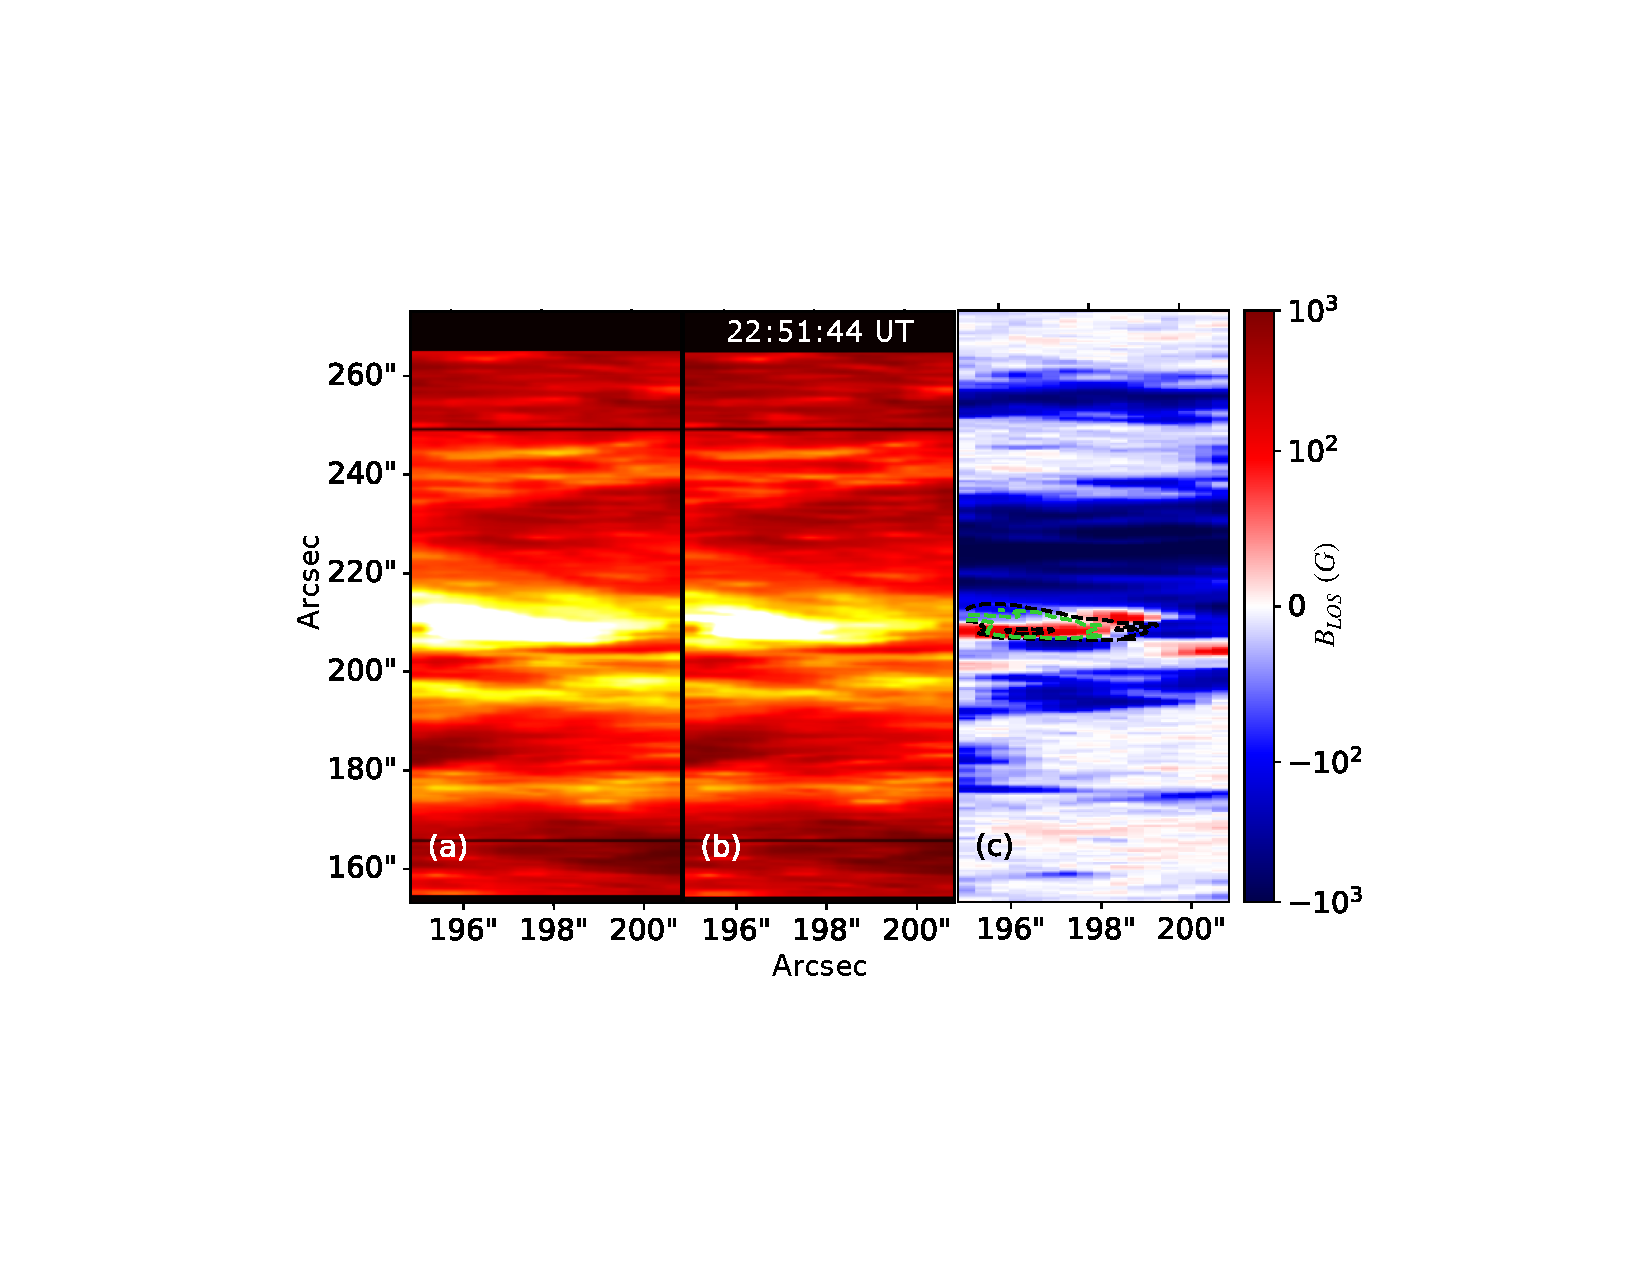
\includegraphics[width=0.5\textwidth,trim={4cm 5cm 4cm 4cm},clip]{Figures/contour_paper_plot_feb-03-2015.pdf}
\caption{Obtained intensity maps in  \ion{Mg}{2}~k (panel a) and h (panel b) lines at the peak of the flare. The rastrered HMI LOS magnetic field density map is shown in panel c. The black and lime green contours on panel c show the contours of  \ion{Mg}{2}~k (panel a) and h (panel b) intensity.}
\label{fig:align_raster_flare3}
\end{figure}
%%--------------------------------------------------

%%--------------------------------------------------
\begin{figure}[ht!]
    \centering
    \includegraphics[trim={2cm 3cm 2cm 3cm},clip,width=0.8\textwidth]{Figures/Feb-04-2015-optical-dep-ev-2.pdf}
    \caption{Time evolution of the  \ion{Mg}{2} k to h line intensity ratio obtained from averaged spectrum over the corresponding magnetic flux bin as labeled for the Feb 3, 2015 flare. Over-plotted red solid line displays the 1{--}8~{\AA} GOES X-ray light curve.}
    \label{fig:optical_dep_ev_c}
\end{figure}
%%--------------------------------------------------

We present the GOES 1{--}8~{\AA}light curve (red solid line) alongside the time evolution of the  \ion{Mg}{2} k to h line intensity ratio averaged within the bins of two different magnetic flux densities as a function of time in Fig.\ref{fig:optical_dep_ev_c}. The  \ion{Mg}{2} k to h line intensity ratio exhibits a similar variation as observed in the M-class flare. It peaks during the impulsive phase (k/h$\sim$ 1.12) and decreases to preflare values (k/h$\sim$ 1.09) during the decay phase of the flare, coinciding with the peak of the GOES light curve. It's worth noting that the change in the  \ion{Mg}{2} k to h line intensity ratio is less pronounced for this flare compared to the M-class event. However, we also observe that the ratio shows a persistent increase from the onset of the flare.

%%--------------------------------------------------
\section{Outlook}
%%--------------------------------------------------

The  \ion{Mg}{2}~k to h line intensity ratios serve as a valuable diagnostic for assessing the opacity of the local plasma and can provide insights into changes in the local plasma environment within the solar chromosphere during flares. In this study, we investigated the temporal variation of  \ion{Mg}{2}k to h line intensity ratios during the evolution of three flares classified as X-class, M-class, and C-class. We also examined the variation of intensity ratios across different magnetic flux density bins, utilizing observations from IRIS and HMI. Co-alignment of IRIS and HMI observations was achieved using 1600{\AA} images recorded by AIA.

It's well-documented that  \ion{Mg}{2} profiles exhibit significant spatial variations within flaring regions \citep{dalda23,panos18}. As we binned the IRIS observations based on magnetic field strength, it's important to note that any spatial variation is averaged out and not addressed in our analysis.

Our findings reveal that  \ion{Mg}{2} k to h line intensity ratios undergo changes during flares. For M-class and C-class flares, the ratio starts increasing at the onset of the flare, peaks roughly halfway through the impulsive phase, and then steeply declines thereafter (see Figs.\ref{fig:optical_dep_ev_m} \& \ref{fig:optical_dep_ev_c}). Moreover, the ratios drop even below pre-flare levels during the later stages of the flare (peak and decline phase). However, this behavior is observed only in M and C-class flares, not in X-class flares.

Our observations did not reveal any correlation between line intensity ratios and magnetic flux density. The line intensity ratios for different magnetic field strengths illustrated in Figs.\ref{fig:optical_dep_ev_m},\ref{fig:align_raster_flare2} right panel,\ref{fig:optical_dep_ev_c} indicate a consistent behavior from weak to strong magnetic field strengths. This suggests that the magnetic field similarly affects both  \ion{Mg}{2}~k and h lines, and such effects cancel out when taking the ratios.

\cite{kerr15} studied  \ion{Mg}{2}~k to h line intensity ratios and their temporal variation for individual pixels in both quiet Sun regions and flare locations. While no change in ratios was observed for the quiet Sun region, variations were noted in flaring pixels, suggesting possible differences in heating conditions between non-flaring and flaring atmospheres. However, no correlated change in the ratio with respect to the flare light curve was observed.

Our results align with those of \cite{kerr15}, wherein they also observe the highest change in the ratio during the impulsive phase of the flare, decreasing before the flare reaches its maximum in GOES 1{--}8~{\AA} observations. Such variations in the ratio may indicate changes in the optical depth of the local medium. During the impulsive phase, decreased optical depth might be attributed to localized heating and chromospheric evaporation, while during the decay phase, increased optical depth could be due to condensation and downflows. However, this interpretation remains speculative, particularly as we did not observe such effects in X-class flares.

The results obtained for M-class and C-class flares can be explained by the aforementioned scenario, but the findings for X-class flares are more ambiguous. We couldn't establish a clear distinction in the general properties of these three flares. Notably, while the C-class flare is confined, both M and X flares are eruptive. Therefore, it's plausible that in X-class flares, energy deposition occurs more impulsively and on a shorter timescale than can be sampled. This high impulsiveness may lead to a greater degree of ionization of the medium compared to the other two flares, as supported by the large number of saturated pixels in the data that were discarded. A more definitive conclusion would necessitate analysis of additional such flares, including numerical and theoretical modeling.

The SUIT has four separate narrow band filters for the Mg window, namely NB2 (Blue wing of  \ion{Mg}{2} k), NB3 ( \ion{Mg}{2} k), NB4 ( \ion{Mg}{2} h) and NB5 (Red wing of  \ion{Mg}{2} h). As mentioned in chapter \ref{c:chap2} SUIT observes the full-disk Sun continuously in NB4 with $\sim$ 1 minute cadence and full-disk observations in all eleven science filters every 90 minutes. With the full disk observations in all science filters, we can investigate the opacity variations continuously across various solar features with a cadence of 90 minutes with the NB3 and NB4 ratio. In flare mode, the observing filter sequence is customizable. With high cadence observations in NB3 and NB4, we can investigate the effect of flare heating on the local plasma environment via its manifestation in opacity.